\documentclass[tikz,border=6pt]{standalone}
\usepackage{fontspec}
\usetikzlibrary{arrows.meta,calc,decorations.pathmorphing,positioning}
\setmainfont{Liberation Sans}
\setsansfont{Liberation Sans}

\definecolor{ink}{HTML}{24313B}
\definecolor{muted}{HTML}{667280}
\definecolor{lineblue}{HTML}{1E5B8C}
\definecolor{teal}{HTML}{2F8F83}
\definecolor{teallight}{HTML}{D9F0ED}
\definecolor{amber}{HTML}{D88924}
\definecolor{amberlight}{HTML}{F7E4C5}
\definecolor{rose}{HTML}{B94A65}
\definecolor{roselight}{HTML}{F2DDE3}
\definecolor{manifold}{HTML}{E8EDF7}
\definecolor{grid}{HTML}{C6D1E4}

\tikzset{
  panel/.style={draw=grid, line width=0.45pt, rounded corners=2pt},
  artery/.style={draw=lineblue, line width=2.1pt, -{Latex[length=2.2mm,width=1.6mm]}, line cap=round, line join=round},
  branch/.style={draw=lineblue, line width=1.7pt, -{Latex[length=2.0mm,width=1.4mm]}, line cap=round, line join=round},
  ghostbranch/.style={draw=lineblue!55, line width=1.2pt, -{Latex[length=1.8mm,width=1.2mm]}, line cap=round, line join=round},
  label/.style={font=\sffamily\footnotesize, text=ink},
  tinylabel/.style={font=\sffamily\scriptsize, text=muted},
  title/.style={font=\sffamily\bfseries\footnotesize, text=ink},
  dot/.style={circle, fill=lineblue, inner sep=1.3pt},
  arrowlink/.style={draw=muted, line width=0.75pt, -{Latex[length=2.3mm,width=1.7mm]}, line cap=round}
}

\begin{document}
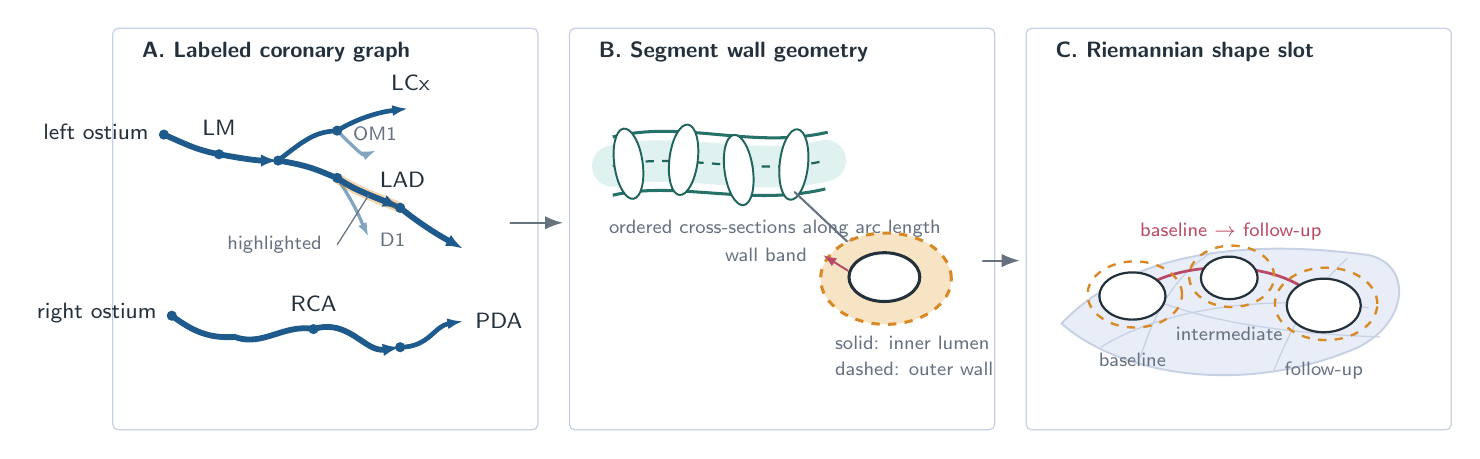
\begin{tikzpicture}[x=1cm,y=1cm]

% Panel frames and titles
\draw[panel] (0,0) rectangle (5.4,5.1);
\draw[panel] (5.8,0) rectangle (11.2,5.1);
\draw[panel] (11.6,0) rectangle (17.0,5.1);
\node[title, anchor=west] at (0.25,4.8) {A. Labeled coronary graph};
\node[title, anchor=west] at (6.05,4.8) {B. Segment wall geometry};
\node[title, anchor=west] at (11.85,4.8) {C. Riemannian shape slot};

% Panel A: simplified coronary tree
\coordinate (lo) at (0.65,3.75);
\coordinate (lm) at (1.35,3.5);
\coordinate (bif) at (2.1,3.42);
\coordinate (lad1) at (2.85,3.2);
\coordinate (lad2) at (3.65,2.82);
\coordinate (lad3) at (4.45,2.3);
\coordinate (lcx1) at (2.85,3.8);
\coordinate (lcx2) at (3.75,4.08);
\coordinate (d1) at (3.25,2.45);
\coordinate (om) at (3.35,3.55);
\draw[artery] (lo) .. controls (0.95,3.62) and (1.05,3.56) .. (lm) .. controls (1.62,3.45) and (1.82,3.42) .. (bif);
\draw[artery] (bif) .. controls (2.55,3.35) and (2.65,3.27) .. (lad1) .. controls (3.05,3.05) and (3.35,2.95) .. (lad2) .. controls (3.95,2.58) and (4.18,2.45) .. (lad3);
\draw[branch] (bif) .. controls (2.48,3.72) and (2.58,3.78) .. (lcx1) .. controls (3.15,3.98) and (3.42,4.04) .. (lcx2);
\draw[ghostbranch] (lad1) .. controls (3.1,2.82) and (3.15,2.66) .. (d1);
\draw[ghostbranch] (lcx1) .. controls (3.1,3.55) and (3.18,3.48) .. (om);
\draw[amber, line width=3.8pt, opacity=0.35, line cap=round] (lad1) .. controls (3.05,3.05) and (3.35,2.95) .. (lad2);
\draw[artery] (lad1) .. controls (3.05,3.05) and (3.35,2.95) .. (lad2);

\coordinate (ro) at (0.75,1.45);
\coordinate (rca1) at (1.55,1.18);
\coordinate (rca2) at (2.55,1.28);
\coordinate (rca3) at (3.65,1.05);
\coordinate (pda) at (4.45,1.38);
\draw[artery] (ro) .. controls (1.02,1.25) and (1.22,1.16) .. (rca1) .. controls (1.9,1.05) and (2.18,1.35) .. (rca2) .. controls (3.0,1.42) and (3.2,0.98) .. (rca3);
\draw[branch] (rca3) .. controls (4.02,1.05) and (4.08,1.32) .. (pda);

\foreach \p in {lo,lm,bif,lad1,lad2,lcx1,ro,rca2,rca3} \node[dot] at (\p) {};
\node[label, anchor=east] at (0.58,3.78) {left ostium};
\node[label, anchor=south] at (1.35,3.62) {LM};
\node[label, anchor=south] at (3.68,2.95) {LAD};
\node[label, anchor=south] at (3.78,4.18) {LCx};
\node[tinylabel, anchor=west] at (3.27,2.42) {D1};
\node[tinylabel, anchor=south] at (3.33,3.55) {OM1};
\node[label, anchor=east] at (0.68,1.48) {right ostium};
\node[label, anchor=south] at (2.55,1.38) {RCA};
\node[label, anchor=west] at (4.48,1.38) {PDA};
\draw[draw=muted, line width=0.45pt] (2.85,2.35) -- (3.25,2.98);
\node[tinylabel, anchor=east] at (2.78,2.35) {highlighted};

% Link A -> B
\draw[arrowlink] (5.05,2.63) -- (5.72,2.63);

% Panel B: tube, ordered cross-sections, and paired contour zoom
\draw[teallight, line width=15pt, opacity=0.85, line cap=round]
  (6.35,3.35) .. controls (7.2,3.55) and (8.15,3.2) .. (9.05,3.42);
\draw[teal!80!black, line width=1.1pt]
  (6.35,3.72) .. controls (7.25,3.94) and (8.12,3.56) .. (9.08,3.78);
\draw[teal!80!black, line width=1.1pt]
  (6.35,2.98) .. controls (7.16,3.17) and (8.1,2.83) .. (9.05,3.06);
\draw[draw=teal!70!black, line width=0.8pt, dashed]
  (6.35,3.35) .. controls (7.2,3.55) and (8.15,3.2) .. (9.05,3.42);

\foreach \x/\y/\a in {6.55/3.38/8,7.25/3.43/-7,7.95/3.30/8,8.65/3.37/-6}
  \draw[draw=teal!70!black, fill=white, line width=0.7pt, rotate around={\a:(\x,\y)}] (\x,\y) ellipse (0.18 and 0.45);
\node[tinylabel, anchor=west] at (6.18,2.55) {ordered cross-sections along arc length};

\draw[arrowlink] (8.66,3.02) -- (9.5,2.23);
\begin{scope}[shift={(9.82,1.92)}]
  \draw[fill=amberlight, draw=none] (0,0) ellipse (0.83 and 0.58);
  \draw[fill=white, draw=none] (-0.02,0.02) ellipse (0.45 and 0.31);
  \draw[draw=amber, dashed, line width=1.1pt] (0,0) ellipse (0.83 and 0.58);
  \draw[draw=ink, line width=1.1pt] (-0.02,0.02) ellipse (0.45 and 0.31);
  \draw[draw=rose, line width=0.7pt, -{Latex[length=1.7mm,width=1.2mm]}] (-0.48,0.1) -- (-0.8,0.3);
  \node[tinylabel, anchor=east] at (-0.88,0.31) {wall band};
\end{scope}
\node[tinylabel, anchor=west] at (9.05,1.1) {solid: inner lumen};
\node[tinylabel, anchor=west] at (9.05,0.78) {dashed: outer wall};

% Link B -> C
\draw[arrowlink] (11.05,2.15) -- (11.52,2.15);

% Panel C: manifold and local shapes
\path[fill=manifold, draw=grid, line width=0.7pt]
  (12.05,1.35) .. controls (12.85,2.2) and (14.25,2.45) .. (15.95,2.22)
  .. controls (16.5,2.1) and (16.47,1.38) .. (15.82,1.05)
  .. controls (14.45,0.45) and (12.85,0.65) .. (12.05,1.35) -- cycle;
\draw[grid, line width=0.45pt]
  (12.55,1.05) .. controls (13.35,1.55) and (14.65,1.72) .. (15.95,1.55);
\draw[grid, line width=0.45pt]
  (12.85,1.82) .. controls (13.75,1.35) and (15.0,1.22) .. (16.1,1.18);
\draw[grid, line width=0.45pt]
  (13.05,0.92) .. controls (13.25,1.55) and (13.52,1.98) .. (13.95,2.25);
\draw[grid, line width=0.45pt]
  (14.75,0.76) .. controls (14.98,1.35) and (15.25,1.78) .. (15.68,2.18);

\coordinate (s1) at (12.95,1.7);
\coordinate (s2) at (14.18,1.93);
\coordinate (s3) at (15.38,1.58);
\draw[draw=rose, line width=1.0pt, -{Latex[length=2.0mm,width=1.5mm]}]
  (s1) .. controls (13.45,2.18) and (14.75,2.18) .. (s3);
\node[tinylabel, text=rose, anchor=south] at (14.2,2.28) {baseline $\rightarrow$ follow-up};

\begin{scope}[shift={(s1)}]
  \draw[fill=white, draw=ink, line width=0.8pt] (0,0) ellipse [x radius=0.42, y radius=0.30];
  \draw[draw=amber, dashed, line width=0.85pt] (0.03,0.02) ellipse [x radius=0.60, y radius=0.42];
\end{scope}
\begin{scope}[shift={(s2)}]
  \draw[fill=white, draw=ink, line width=0.8pt] (0,0) ellipse [x radius=0.36, y radius=0.27];
  \draw[draw=amber, dashed, line width=0.85pt] (0.03,0.02) ellipse [x radius=0.54, y radius=0.39];
\end{scope}
\begin{scope}[shift={(s3)}]
  \draw[fill=white, draw=ink, line width=0.8pt] (0,0) ellipse [x radius=0.47, y radius=0.34];
  \draw[draw=amber, dashed, line width=0.85pt] (0.03,0.02) ellipse [x radius=0.65, y radius=0.46];
\end{scope}
\node[tinylabel, anchor=north] at (12.95,1.1) {baseline};
\node[tinylabel, anchor=north] at (14.18,1.43) {intermediate};
\node[tinylabel, anchor=north] at (15.38,0.98) {follow-up};

\end{tikzpicture}
\end{document}
